% !TeX program = xelatex
% A LaTeX thesis template for Fudan University.
% Author：qq
% SPDX-FileCopyrightText: 2026 qq
% SPDX-License-Identifier: GPL-3.0-only
%
% 在本目录运行 latexmk -xelatex main.tex，自动更新目录、交叉引用和参考文献。

% 使用项目内的宋体时，取消下一行注释，并填入实际路径和文件名（区分大小写）。
% \AddToHook{fduthesis/cjk-font}{\setCJKmainfont[Path=fonts/,FontIndex=0,AutoFakeBold=2]{simsun.ttc}}
\documentclass{fduthesis}

% 在 PDF 末尾生成书脊打印页。
% \makespine

\usepackage{amsmath}
% 中文字号换算为 TeX pt 后常有小数，按实际字号缩放数学扩展字体。
\DeclareFontShape{OMX}{cmex}{m}{n}{<-7.5>cmex7<7.5-8.5>cmex8<8.5-9.5>cmex9<9.5->cmex10}{}

\usepackage{booktabs}

% algorithm.sty 的版权注释使用 Latin-1，加载完毕后恢复 XeTeX 的自动编码检测。
\ifdefined\XeTeXdefaultencoding
  \AddToHook{file/algorithm.sty/before}{\XeTeXdefaultencoding "ISO-8859-1"\relax}
  \AddToHook{file/algorithm.sty/after}{\XeTeXdefaultencoding "auto"\relax}
\fi
\usepackage{algorithm,algpseudocode}

\usepackage{listings}
% 显示代码行号：取消下一行注释。
% \lstset{numbers=left}
% 启用语法高亮：取消下一行注释，并在代码清单中指定 language（如 Python）。
% \lstset{keywordstyle=\color{blue},keywordstyle=[2]\color{blue},commentstyle=\itshape,stringstyle=\color{red}}

% 参考文献后端二选一，并在正文结束处启用对应的输出命令。
% 默认使用 BibTeX
\usepackage[uppercasefamily=false]{gbt7714}
\bibliographystyle{gbt7714-2025-numeric}

% 启用 biblatex + Biber， 取消下两行的注释，并在正文结束处启用 \printbibliography。
% \usepackage[backend=biber,style=gb7714-2025]{biblatex}
% \addbibresource{reference.bib}

\fdusetup{
  % 正文页码默认从 1 起编。取消下一行注释可从 i 起编。
  % main-page-numbering = roman,
  % 页眉样式可改为 centered（章标题居中）或 outer（正文页眉靠外侧）。
  header-style = alternating,
  %
  % 图表编号默认使用点号（图 1.1）。改用短横线时，取消下一行注释。
  % figure-table-separator = hyphen,
  % 正文和附录的公式编号统一使用点号。改用短横线时，取消下一行注释。
  % equation-separator = hyphen,
  %
  % 学位类别：学术学位填 academic，专业学位填 professional。
  type = academic,
  % 学位层次：本科填 bachelor，硕士填 master，博士填 doctor。
  degree = doctor,
  %
  title = {有序数组查找的比较次数分析},
  title-en = {Comparison Counts for Search in Sorted Arrays},
  %
  author = {张三}, student-id = {123456789},
  % 同等学力人员填“同等学力人员”，其他学生填 none。“英文项目”由 lang=en 自动添加。
  student-category = none,
  %
  supervisor = {李四}, supervisor-title = {教授},
  committee = {李四教授, 王五副教授},
  %
  major = {计算机科学与技术}, department = {计算与智能创新学院},
  date = {2026\hspace{0.5em}年\hspace{0.5em}6\hspace{0.5em}月\hspace{0.5em}30\hspace{0.5em}日},
  % 中图分类号。请到 https://www.clcindex.com/ 按论文主题查询。
  clc = {TP301},
  %
  keywords = {有序数组, 二分查找, 算法分析},
  keywords-en = {sorted arrays, binary search, algorithm analysis},
  %
  % 非涉密论文填 none，封面不显示密级；涉密论文填写经核定的密级和保密期限。
  secret-level = {none},
}

\begin{document}

% --- 前置部分 ---
\frontmatter

% 封面
\makecoverpage
% 指导小组
\makecommittee

% 目录
% 若希望目录只列到“一级节标题”（如 1.1），取消下一行注释
% \setcounter{tocdepth}{1}
\tableofcontents

% 中文摘要
\begin{fdusummary}
在升序数组中定位一个键，二分查找可以不断排除一半的候选元素，顺序查找却可能在第一步就命中。哪一种方法平均比较的次数更少，取决于查询落在数组的什么位置。本文固定一个含七个互异整数的数组，以目标键和被访问元素的一次三路比较为单位，逐键记录两种算法的查找路径。由判定树可知，二分查找最多比较三次；若七个键等概率出现，顺序查找与二分查找的平均比较次数分别为 $4$ 和 $17/7$。随后保持数组顺序不变，逐步提高首键的查询概率，并将其余查询均匀分配给另外六个键。两种方法的平均代价在首键概率达到 $13/25$ 时相等，超过这一比例后，顺序查找的平均比较次数更少。最后用空数组、边界命中与查找失败三类输入核对实现，区分返回下标和比较次数这两个容易混淆的量。
\end{fdusummary}

% 英文摘要
\begin{fdusummaryen}
Binary search halves the candidate interval after each unsuccessful comparison, yet a
linear scan can find its target on the first probe. We compare the two methods on a
sorted array of seven distinct keys, counting one three-way comparison per probe.
With uniformly distributed successful queries, a linear scan takes four comparisons
on average, against $17/7$ for binary search. We then assign probability $p$ to the
first key and divide the remaining probability equally among the other six keys.
The expected costs coincide at $p=13/25$. Above that threshold the linear scan uses
fewer comparisons, even though binary search still has the smaller worst-case cost.
Boundary cases illustrate how to distinguish a valid index of zero from a failed lookup.
\end{fdusummaryen}

% 图表清单页
\listoffigures
\listoftables

%--- 进入正文 ---
\mainmatter
% 如需隐藏每章首页的页眉和横线，取消下一行注释。页脚保留页码。
% \ctexset{chapter/pagestyle=plain}

\chapter{有序数组的查找代价}
一份已经按学号排好的名册，可以从第一行开始逐行核对，也可以先翻到中间，
根据学号的大小决定接着查哪一半。假如要找的人恰在第一行，逐行核对只看一个名字就够了；
假如他在最后一行，两种查法要看的名字数可能相差很大。本章把名册简化为有序数组，
先比较查到指定键各需几步，再考察数组增加一个元素时，最长的查找路径会怎样变化。

\section{比较次数的定义}
设数组按升序存储 $n$ 个互异的键。顺序查找从第一个元素向后扫描；
二分查找取当前区间的中点，根据比较结果保留左半区间或右半区间\cite{knuth1998}。
本文将目标键与一个数组元素的三路比较计为一次。%
\footnote{三路比较一次返回小于、等于或大于。若用两个条件判断实现，执行的判断指令数可能不同。}
例如在名册中查学号 5，看到学号 4 就足以决定向后找。移动下标、计算中点和检查循环条件
均不额外计数。这里假定名册在查询前已经排好序，排序的工作也不计入单次查找。

一次未命中的中点比较至多留下 $\lfloor n/2\rfloor$ 个候选键。
因此，对非空数组，两种方法在成功查找时的最坏比较次数分别为
\begin{equation}
  C_{\mathrm{seq}}(n)=n,\qquad C_{\mathrm{bin}}(n)=\lfloor\log_2 n\rfloor+1 .
  \label{eq:worst}
\end{equation}

\subsection{按查询键计数}
对数组 $[1,2,3,4,5,6,7]$，表~\ref{tab:counts} 列出各键从开始查找到首次命中的比较次数。
两行的最大值分别为 7 和 3，与式（\ref{eq:worst}）一致。
% 表题置于表上方。图、表的 \label 紧跟 \caption，以取得正确编号。
\begin{table}[htbp]
  \centering
  \caption{查找不同目标键所需的比较次数}
  \label{tab:counts}
  \begin{tabular}{lrrrrrrr}
    \toprule
    目标键 & 1 & 2 & 3 & 4 & 5 & 6 & 7 \\
    \midrule
    顺序查找 & 1 & 2 & 3 & 4 & 5 & 6 & 7 \\
    二分查找 & 3 & 2 & 3 & 1 & 3 & 2 & 3 \\
    \bottomrule
  \end{tabular}
\end{table}

表中第一行的数值恰好等于键值，这是选用连续整数所产生的巧合。若将七个键分别改为
$10,20,\ldots,70$，查找 50 仍要顺序访问五个元素。对二分查找也一样：
比较的对象从 4、6、5 变为 40、60、50，每一步的大小关系都保持原样。
因此，在互异键之间，只要知道目标在数组中排第几，就能复用表中的结果。

\section{沿判定树查找}
算法~\ref{alg:binary-search} 从下标 0 开始，以 $l$ 和 $r$ 标出尚待检查的第一个和
最后一个位置。如果区间长度为偶数，两个中央位置都可以作为中点；本文统一选靠左的一个。
这个约定使读者可以根据数组重建同一棵判定树，也可以用附录中的代码~\ref{lst:binary-search}
逐步核对访问顺序。

\begin{algorithm}[htbp]
  \caption{有序数组的二分查找}\label{alg:binary-search}
  \begin{algorithmic}
    \Require 升序数组 $A$，目标键 $x$
    \State $l \gets 0,\quad r \gets |A|-1$
    \While{$l \le r$}
      \State $m \gets \lfloor (l+r)/2 \rfloor$
      \If{$A[m]=x$}
        \State \Return $m$
      \ElsIf{$A[m]<x$}
        \State $l \gets m+1$
      \Else
        \State $r \gets m-1$
      \EndIf
    \EndWhile
    \State \Return \texttt{None}
  \end{algorithmic}
\end{algorithm}

图~\ref{fig:search} 中的节点标的是键值。从父节点走向子节点，表示上一次比较排除了
一部分候选键。以查找键 5 为例：
\begin{enumerate}
  \item 先与根节点 4 比较，因 $5>4$，保留区间 $[5,7]$。
  \item 再与中点 6 比较，因 $5<6$，剩下的区间只含键 5。
  \item 与键 5 比较并命中，整个过程共比较三次。
\end{enumerate}
\begin{figure}[htbp]
  \centering
  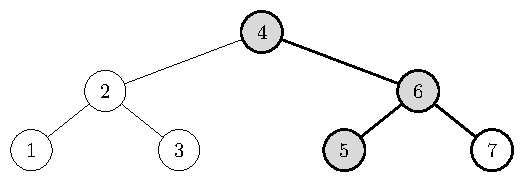
\includegraphics[width=.65\linewidth]{figures/figure1.pdf}
  \caption{二分查找判定树，灰色节点标出查找键 5 的路径}
  \label{fig:search}
\end{figure}
把同一条路径写成下标，就能看清每次排除的范围。第一次访问下标 3，读到键 4；
由于数组升序，下标 0 至 3 的元素都小于 5，可以一并排除。第二次访问下标 5，
读到键 6，此时下标 5 和 6 都可排除。余下的下标 4 正好存着键 5。这个例子也说明
了为什么循环条件要包含 $l=r$：两端重合时仍有一个候选元素有待检查。

\section{数组增长时的最坏代价}
\subsection{从七个键到八个键}
在数组末尾添上键 8，再按相同的中点规则查找。第一次访问的仍是键 4，右边却多了
一个候选键。若目标为 8，后续依次访问 6、7、8，至此共比较四次。
若目标为 1，后续仍访问 2、1，和原先完全相同。新增的这一次比较只出现在通向
新键的路径上，却足以把整棵树的最大层数从三层推到四层。

为什么无法把八个键都放在前三层？第一次比较最多让一个键直接命中。比较结果若为
小于或大于，第二次比较各能再让一个键命中。到第三次，留给命中的位置最多还有四个。
合计 $1+2+4=7$ 个位置，恰好容纳原数组的全部键。即便重新选择各个中点，第八个键
的加入也意味着至少有一个键需要第四次比较。

\subsection{从树高估计查找预算}
同样的计数可以推广到任意层数。设每次查询最多允许比较 $h$ 次，把根节点算作
第一层，第 $i$ 层至多有 $2^{i-1}$ 个可命中的键。因此，在预算内能够区分的键数至多为
\begin{equation}
  N(h)=\sum_{i=1}^{h}2^{i-1}=2^h-1 .
  \label{eq:tree-capacity}
\end{equation}
反过来，要让 $n$ 个互异键都能在预算内找到，至少需要
$h=\lceil\log_2(n+1)\rceil$ 层。对正整数 $n$，这正好等于
式（\ref{eq:worst}）中的 $\lfloor\log_2 n\rfloor+1$。逐次取中点的二分查找达到了这个下界。

例如，九次比较最多容纳 $2^9-1=511$ 个键，十次则可容纳 $2^{10}-1=1023$ 个键。
因此，一份有 1000 个学号的名册，用二分查找至多核对十个学号就能找到其中任何一人。
若依据这个预算估计一天的总核对次数，就要留意查询落在哪里：查十次根节点和查十次
最深层的键，工作量可以相差十倍。下一章回到七个键的数组，用各键的查询频率计算平均代价。

\chapter{查询分布如何改变平均代价}
\section{让首键成为热点}
假设这七个键是按编号排好的七个菜单项。若第一项是最常用的操作，从头扫描未必吃亏。
为把这个直觉变成可检验的结论，记首键被查询的概率为 $p$，另外六个键各占 $(1-p)/6$。
全过程只改变查询频率，数组顺序和算法~\ref{alg:binary-search} 的中点选择规则保持一致。

表~\ref{tab:counts} 给出了所需的全部数据。查询首键时，顺序查找只比较一次，
二分查找要依次访问 4、2、1。查询其余六个键时，顺序查找的比较次数之和为 27，
二分查找为 14。按这两类查询分别加权，得到
\begin{equation}
  \begin{aligned}
    E_{\mathrm{seq}}(p) &= p + (1-p)\,27/6 = (9-7p)/2, \\
    E_{\mathrm{bin}}(p) &= 3p + (1-p)\,14/6 = (7+2p)/3 .
  \end{aligned}
  \label{eq:weighted-cost}
\end{equation}
这里有两个方便的自检点。取 $p=1/7$ 时，所有键恢复等概率，代回式（\ref{eq:weighted-cost}）
应得到摘要中的两个均值。取 $p=1$ 时，每次都查首键，结果应分别退化为 1 和 3。

\section{交点及其含义}
图~\ref{fig:weighted-cost} 中，顺序查找的直线向下倾斜，二分查找的直线却略微上升。
这是因为首键位于二分判定树的第三层：增加它的权重，会把原本落在根节点或第二层的
一部分查询移到更深处。令两条直线的纵坐标相等，解得 $p=13/25$，交点处平均比较
$67/25$ 次。表~\ref{tab:weighted-cost} 给出三个可以手算核对的位置。

\begin{figure}[htbp]
  \centering
  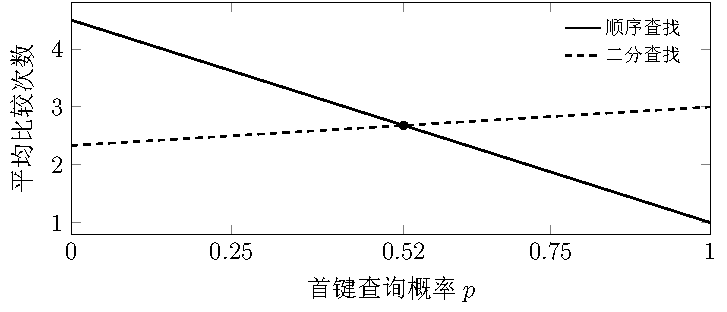
\includegraphics{figures/figure2.pdf}
  \caption{首键查询概率与平均比较次数的关系}\label{fig:weighted-cost}
\end{figure}

\begin{table}[htbp]
  \centering
  \caption{三种查询分布下的平均比较次数}\label{tab:weighted-cost}
  \begin{tabular}{lccc}
    \toprule
    查询分布 & 首键概率 & 顺序查找 & 二分查找 \\
    \midrule
    七个键等概率 & $1/7$   & $4$     & $17/7$  \\
    两种代价相等 & $13/25$ & $67/25$ & $67/25$ \\
    只查询首键   & $1$     & $1$     & $3$     \\
    \bottomrule
  \end{tabular}
\end{table}

这个交点依赖热点的位置。若把热点从键 1 换成键 4，二分查找在第一次比较时就能返回，
顺序查找则要走到第四个位置。因此，把分析用于另一组查询时，需要同时知道热点的频率
及其在数组中的位置。这里计算的是访问元素的次数；若要估计运行时间，还需测量每次
访问和分支判断的实际开销。

\section{查找失败时如何计数}
前面的平均值都以成功命中为前提。若目标不在数组里，它可能小于首键、大于末键，
也可能落在相邻两键之间。七个互异的键将数轴分成八个这样的空档。
例如，查询 $4.5$ 时，二分查找先后访问 4、6、5，第三次比较后区间为空。
图~\ref{fig:search} 的叶节点都在第三层，因此无论目标在哪个空档，查找失败都恰好访问三个元素。

顺序查找可以利用升序条件提前停止：一旦遇到大于目标的键，后面的元素也无需检查。
从左到右看八个空档，访问次数依次为 $1,2,3,4,5,6,7,7$。末尾两个数相同，
是因为无论目标略小于 7 还是大于 7，都必须读到数组末端。
若八个空档等概率出现，顺序查找的失败代价为 $35/8$。由此可见，报告一个平均值时，
需要交代统计对象是成功查询、失败查询，还是按特定比例混合的查询。

% --- 正文结束 ---

% 参考文献：按导言区选用的后端启用其中一行。
\bibliography{reference} % 默认使用 BibTeX
% \printbibliography    % 启用 biblatex + Biber

% 进入附录，章编号改用 A、B、C……
\appendix
\chapter{计算与实现核对}\label{app:average}
\section{等概率情形的逐层求和}
假设每次查询都成功，且七个键被查询的概率均为 $1/7$。
顺序查找的平均比较次数为 $(1+2+3+4+5+6+7)/7=4$。
在二分查找判定树中，第一、二、三层各有一、二、四个节点，
故平均比较次数为 $(1\times1+2\times2+4\times3)/7=17/7$。

\section{边界输入与返回值}
代码~\ref{lst:binary-search} 使用闭区间。循环开始时，如果目标存在，它的下标必在
$[l,r]$ 内。当区间缩成单个位置时仍须比较一次，因此循环条件包含等号。
若某一轮未命中，更新后的区间至少少一个元素；当左端点超过右端点，函数返回
\texttt{None}。这个约定使调用者能够区分查询失败与恰好命中下标 0。

\begin{lstlisting}[language=Python,caption={二分查找的 Python 实现},label={lst:binary-search}]
def binary_search(keys, target):
    lo, hi = 0, len(keys) - 1
    while lo <= hi:
        mid = (lo + hi) // 2
        if keys[mid] == target:
            return mid
        if keys[mid] < target:
            lo = mid + 1
        else:
            hi = mid - 1
    return None
\end{lstlisting}

\section{按预期结果检查实现}
表~\ref{tab:boundary} 给出四个可直接传入函数的例子。最后一例查询两个相邻键之间的值：
先比较 3，再比较 1，随后区间变空。返回值与空数组一样，走到返回语句的路径却不同。
\begin{table}[htbp]
  \centering
  \caption{二分查找的边界输入与预期结果}\label{tab:boundary}
  \begin{tabular}{llccc}
    \toprule
    情形 & 输入数组 & 目标键 & 返回值 & 访问元素次数 \\
    \midrule
    空数组   & $[\,]$  & 2 & \texttt{None} & 0 \\
    命中首键 & $[1,3,5]$ & 1 & 0 & 2 \\
    命中末键 & $[1,3,5]$ & 5 & 2 & 2 \\
    键间缺值 & $[1,3,5]$ & 2 & \texttt{None} & 2 \\
    \bottomrule
  \end{tabular}
\end{table}

代码~\ref{lst:boundary-tests} 可接在函数定义之后运行。断言分别检查返回值的含义和
成功时的具体下标。如果把循环条件从 $l\le r$ 改成 $l<r$，查找会跳过最后一个候选位置，
两个端点用例就会暴露这一错误。

\begin{lstlisting}[language=Python,caption={边界输入的断言检查},label={lst:boundary-tests}]
keys = [1, 3, 5]
assert binary_search([], 2) is None
assert binary_search(keys, 1) == 0
assert binary_search(keys, 5) == 2
assert binary_search(keys, 2) is None
\end{lstlisting}

% 附录结束，切换到无编号的后置部分
\backmatter

% 致谢
\begin{acknowledgements}
感谢导师对查找算法示例和图表表达提出的建议。
\end{acknowledgements}

% 声明页
\makeauthorization

\end{document}
